\documentclass[11pt]{article}
\usepackage{pifont}
\usepackage{multicol}
\usepackage{listings}
\usepackage{pgf}
\usepackage{tikz}
\usepackage{alltt}
\usepackage{hyperref}
\usepackage{url}
\usepackage{amssymb}
\usetikzlibrary{arrows,automata,shapes,positioning}
\tikzstyle{block} = [rectangle, draw, fill=blue!20, 
    text width=5em, text centered, rounded corners, minimum height=2em]
\tikzstyle{bt} = [rectangle, draw, fill=blue!20, 
    text width=1em, text centered, rounded corners, minimum height=2em]
\newcommand{\xmark}{\ding{55}}

\newtheorem{defn}{Definition}
\newtheorem{crit}{Criterion}
\newcommand{\true}{\mbox{\sf true}}
\newcommand{\false}{\mbox{\sf false}}

\newcommand*\circled[1]{\tikz[baseline=(char.base)]{
            \node[shape=circle,draw,inner sep=2pt] (char) {#1};}}


\newcommand{\handout}[5]{
  \noindent
  \begin{center}
  \framebox{
    \vbox{
      \hbox to 5.78in { {\bf Software Testing, Quality Assurance and Maintenance } \hfill #2 }
      \vspace{4mm}
      \hbox to 5.78in { {\Large \hfill #5  \hfill} }
      \vspace{2mm}
      \hbox to 5.78in { {\em #3 \hfill #4} }
    }
  }
  \end{center}
  \vspace*{4mm}
}

\newcommand{\lecture}[4]{\handout{#1}{#2}{#3}{#4}{Lecture #1}}
\topmargin 0pt
\advance \topmargin by -\headheight
\advance \topmargin by -\headsep
\textheight 8.9in
\oddsidemargin 0pt
\evensidemargin \oddsidemargin
\marginparwidth 0.5in
\textwidth 6.5in

\parindent 0in
\parskip 1.5ex
%\renewcommand{\baselinestretch}{1.25}

\usepackage{enumitem}

\newtheorem{prop}{Proposition}
\newtheorem{lemma}{Lemma}
\usepackage{ebproof}
\newcommand{\qedsymbol}{\rule{1ex}{1ex}}

\lstset{ %
language=Java,
basicstyle=\ttfamily,commentstyle=\scriptsize\itshape,showstringspaces=false,breaklines=true,numbers=left}

%\usepackage{fontspec}
%\setmonofont{Cousine}[Scale=MatchLowercase]

\begin{document}

\lecture{7 --- January 27, 2025}{Winter 2025}{Patrick Lam}{version 1b}

Here's a function.

\begin{lstlisting}
def Foo(x,y):
""" requires: x and y are int
    ensures: returns floor(max(x,y)/min(x,y))"""
  if x > y:
    return x / y
  else:
    return y / x
\end{lstlisting}

We are going to use \emph{symbolic execution} to automatically generate a test suite that:
\begin{itemize}[noitemsep]
\item achieves full branch coverage (actually even better: full path coverage);
\item identifies dead code; and,
\item discovers whether division by 0 is possible.
\end{itemize}

\paragraph{Symbolic Execution in a Nutshell.} In four steps:
\begin{enumerate}[noitemsep]
\item \emph{transform} the program to add explicit tests for division by 0 (oracles);
\item \emph{traverse} the program to compute each program path; \\
  \hspace*{2em} path1: \texttt{x > y, y == 0}; path2: \texttt{x > y, y != 0, return x / y}; etc.
\item \emph{solve} constraints for each path using a constraint (or logic) solver; \\
  \hspace*{2em} path1: \texttt{x=10,y=0}; path2: \texttt{x=10,y=1}; etc.
\item \emph{run} the program on tests generated by the previous step.
\end{enumerate}
Under symbolic execution, all testing is now automatic. And, for some definitions of exhaustive (path coverage), the testing is also exhaustive.

Here's the transformed program.
\begin{lstlisting}
def Foo(x,y):
""" requires: x and y are int
    ensures: returns floor(max(x,y)/min(x,y))"""
  if x > y:
    assert y != 0
    return x / y
  else:
    assert x != 0
    return y / x
\end{lstlisting}

\paragraph{Main Components of Symbolic Execution.} As above, we have:

\emph{Traversing}: automatically exploring program paths, executing the program on symbolic input values (vs the concrete values that the semantics operates on); forking execution at each branch; and recording branching conditions.

\emph{Solving constraints}: deciding path feasibility, and generating test cases to get paths and to find bugs.

\paragraph{Traversing Paths.} Let's enumerate all of the paths.
\begin{enumerate}[noitemsep]
\item \texttt{x > y, y == 0}: assertion fails
\item \texttt{x > y, y != 0}: reaches \texttt{return x / y}
\item \texttt{x <= y, x == 0}: assertion fails
\item \texttt{x <= y, x != 0}: reaches \texttt{return y / x}
\end{enumerate}

\paragraph{Solving Constraints.} For each path, we generate a set of constraints and ask z3 to solve them for us:
\begin{lstlisting}
(declare-fun x () Int)
(declare-fun y () Int)
(assert (> x y))
(assert (not (= y 0)))
(check-sat)
(get-model)
\end{lstlisting}

\section*{History of symbolic execution}
Symbolic execution is actually quite old; here are references from 1975 by Robert S. Boyer, Bernard Elspas, and Karl N. Levitt; and James C. King: \cite{boyer75:_selec,king75}.

\begin{quote}
  Recent work on proving the correctness of programs by formal analysis [5] shows great promise and appears to be the ultimate technique for producing reliable programs. However,
  the practical accomplishments in this area fall short of a tool for routine use. Fundamental problems in reducing the theory to practice are not likely to be solved in the immediate future.
\end{quote}

I will also point out that even if the software works perfectly (never crashes, for instance), you still don't know that the software is doing the right thing. You need SE 463 (requirements)
for that.

In any case, in the 2000s, SAT solvers and their big brothers SMT solvers made SAT feasible in practice. In the context of formal verification, constraint solving is easy. Classical verification
algorithms---with worst-case exponential running time---became viable in practice even if not in theory.

There were also conceptual breakthroughs in the mid-2000s with dynamic symbolic execution, which we'll see in Lecture 9.

\section*{Symbolic Execution Illustrated}
Let's continue with an example.
\begin{lstlisting}
  int max4(int a, int b, int c, int d) {
    return max2(max2(a, b /*(1)*/), max2(c, d /*(2)*/) /*(3)*/);
  }

  int max2(int x, int y) {
    if (x <= y) return y;
    else return x;
  }
\end{lstlisting}
We can exhaustively explore all of the paths. Hereafter, $\mathit{pc}$ means path condition (rather than program counter as before), and it's the thing inside the boxes. Solid lines are the true branch, while dashed lines are the false branch.
This tree is different from the one in the slides, but I think it's right. Each node shows the result of the previous test. In this picture (and only in this picture---for space reasons), you get
the path condition by conjoining the conditions that lead to your path; for instance, the full path condition at the left-most leaf is $a \le b \wedge c \le d \wedge b \le d$.

\begin{center}
    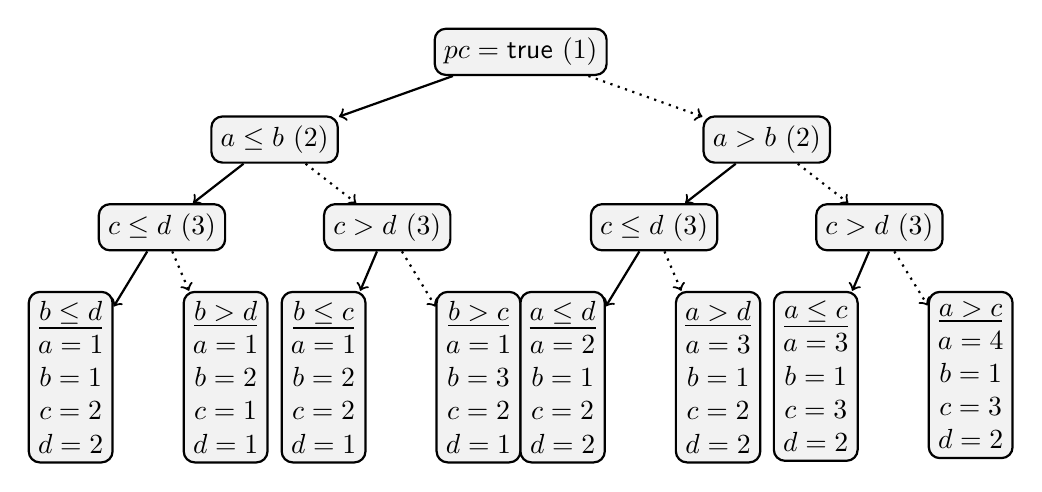
\begin{tikzpicture}[
        node distance=.5cm and .5cm,
        every node/.style={draw, rounded corners, fill=gray!10, align=center},
        every path/.style={thick},
        decision/.style={draw, rounded corners, fill=gray!20, align=center, minimum width=3.5cm, yshift=2em}
    ]

    % Nodes
      \node (start) {$pc = \textsf{true}$ (1)};
      \node (l)[below left=of start,xshift=-2em] {$a \le b$ (2)};
      \node (r)[below right=of start,xshift=2em] {$a > b$ (2)};
      
      \node (ll)[below left=of l,xshift=2em] {$c \le d$ (3)};
      \node (lr)[below right=of l,xshift=-2em] {$c > d$ (3)};
      \node (rl)[below left=of r,xshift=2em] {$c \le d$ (3)};
      \node (rr)[below right=of r,xshift=-2em] {$c > d$ (3)};

      \node (lll)[below left=of ll,xshift=2em]   {\underline{$b \le d$} \\ $a=1$\\$b=1$\\$c=2$\\$d=2$};
      \node (llr)[below right=of ll,xshift=-3em] {\underline{$b > d$} \\ $a=1$\\$b=2$\\$c=1$\\$d=1$};
      \node (lrl)[below left=of lr,xshift=3em]   {\underline{$b \le c$} \\ $a=1$\\$b=2$\\$c=2$\\$d=1$};
      \node (lrr)[below right=of lr,xshift=-2em] {\underline{$b > c$} \\ $a=1$\\$b=3$\\$c=2$\\$d=1$};

      \node (rll)[below left=of rl,xshift=2em]   {\underline{$a \le d$} \\ $a=2$\\$b=1$\\$c=2$\\$d=2$};
      \node (rlr)[below right=of rl,xshift=-3em] {\underline{$a > d$} \\ $a=3$\\$b=1$\\$c=2$\\$d=2$};
      \node (rrl)[below left=of rr,xshift=3em]   {\underline{$a \le c$} \\ $a=3$\\$b=1$\\$c=3$\\$d=2$};
      \node (rrr)[below right=of rr,xshift=-2em] {\underline{$a > c$} \\ $a=4$\\$b=1$\\$c=3$\\$d=2$};
      
    \draw[->] (start) -- (l);
    \draw[->, dotted] (start) -- (r);
    
    \draw[->] (l) -- (ll);
    \draw[->, dotted] (l) -- (lr);
    \draw[->] (r) -- (rl);
    \draw[->, dotted] (r) -- (rr);

    \draw[->] (ll) -- (lll);
    \draw[->,dotted] (ll) -- (llr);
    \draw[->] (lr) -- (lrl);
    \draw[->,dotted] (lr) -- (lrr);

    \draw[->] (rl) -- (rll);
    \draw[->,dotted] (rl) -- (rlr);
    \draw[->] (rr) -- (rrl);
    \draw[->,dotted] (rr) -- (rrr);
    
    \end{tikzpicture}
\end{center}

I manually worked out these test cases to meet the constraints, but of course we can also get z3 to compute it too.
That's the whole reason we're talking about this.

\begin{lstlisting}
(declare-fun a () Int)
(declare-fun b () Int)
(declare-fun c () Int)
(declare-fun d () Int)
(assert (< 0 a))
(assert (< 0 b))
(assert (< 0 c))
(assert (< 0 d))
(assert (<= a b)) 
(assert (> c d))
(assert (<= b c))
(check-sat)
(get-model)
\end{lstlisting}

If you run this, then you get:
\begin{lstlisting}
sat
(
  (define-fun d () Int
    1)
  (define-fun a () Int
    1)
  (define-fun c () Int
    2)
  (define-fun b () Int
    1)
)
\end{lstlisting}

\section*{A Symbolic Execution Example}
We are now going to illustrate how symbolic execution works on this code:
\begin{lstlisting}
  int proc(int x) {
    int r = 0;

    if (x > 8) { // (1)
      r = x - 7
    }

    if (x < 5) { // (2)
      r = x - 2;
    }
  }

\end{lstlisting}

The initial symbolic state, after executing \texttt{r=0}, is this:
\begin{center}
    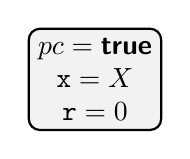
\begin{tikzpicture}[
        node distance=1.5cm and 1cm,
        every node/.style={draw, rounded corners, fill=gray!10, align=center},
        every path/.style={thick},
        decision/.style={draw, rounded corners, fill=gray!20, align=center, minimum width=3.5cm}
    ]


    % Nodes
      \node (start) {\textbf{$pc = \textsf{true}$} \\
        $\texttt{x} = X$ \\
        $\texttt{r} = 0$ };
    
    
    \end{tikzpicture}
\end{center}
The start of the method is always reachable, so \textbf{$pc = \textsf{true}$}. There is one input $X$
stored in program variable $\texttt{x}$. We also know that \texttt{r} is 0 after its initialization.

Program point (1) is a branch, so there are two possible symbolic states coming out of the branch statement.
The path condition is what has to be true to reach a particular point. In this case, on the true branch, it must be
the case that $X > 8$ (that's how you get there); and conversely for the false branch, $X \le 8$. We encode that in the
path condition. In these pictures we use the convention that the solid line denotes the then-branch, while the dotted line
denotes the else-branch.

\begin{center}
    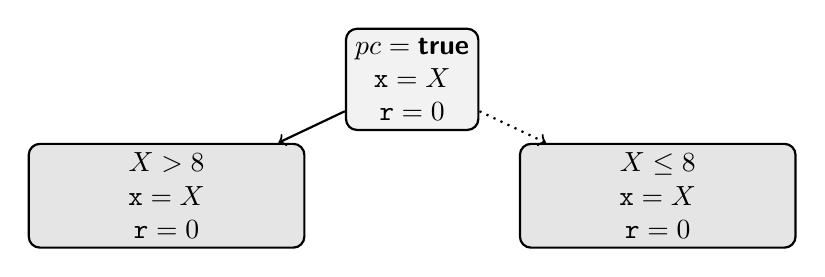
\begin{tikzpicture}[
        node distance=.5cm and .5cm,
        every node/.style={draw, rounded corners, fill=gray!10, align=center},
        every path/.style={thick},
        decision/.style={draw, rounded corners, fill=gray!20, align=center, minimum width=3.5cm}
    ]


    % Nodes
      \node (start) {\textbf{$pc = \textsf{true}$} \\
        $\texttt{x} = X$ \\
        $\texttt{r} = 0$ };
    
    \node (left)[below left=of start, decision,yshift=1em] {$X > 8$ \\ 
        $\texttt{x} = X$ \\
        $\texttt{r} = 0$ };

    \node (right)[below right=of start, decision,yshift=1em] {$X \leq 8$ \\ 
        $\texttt{x} = X$ \\
        $\texttt{r} = 0$ };

    % Edges
      
    \draw[->] (start) -- (left);
    \draw[->, dotted] (start) -- (right);
    
    \end{tikzpicture}
\end{center}
We ask the SAT solver if both path conditions $X > 8$ and $X \le 8$ are satisfiable. They are ($\checkmark$).

We continue executing the code in the then-branch, updating \texttt{r} with its new symbolic value, $X - 7$.
\begin{center}
    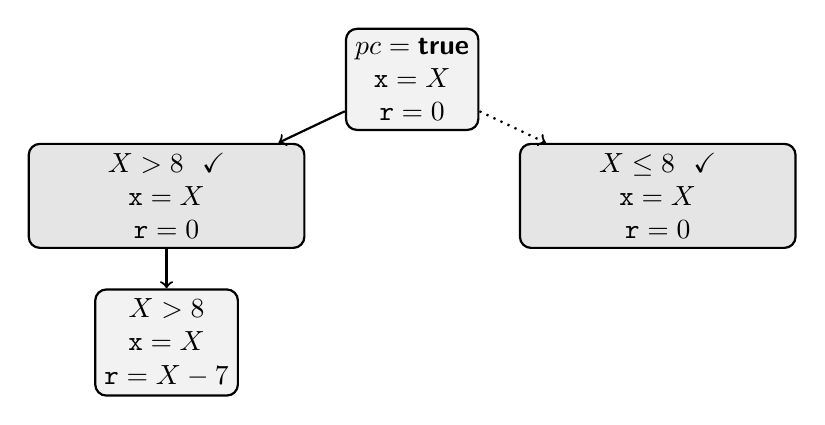
\begin{tikzpicture}[
        node distance=.5cm and .5cm,
        every node/.style={draw, rounded corners, fill=gray!10, align=center},
        every path/.style={thick},
        decision/.style={draw, rounded corners, fill=gray!20, align=center, minimum width=3.5cm}
    ]


    % Nodes
      \node (start) {\textbf{$pc = \textsf{true}$} \\
        $\texttt{x} = X$ \\
        $\texttt{r} = 0$ };
    
    \node (left)[below left=of start, decision,yshift=1em] {$X > 8$~~$\checkmark$ \\ 
        $\texttt{x} = X$ \\
        $\texttt{r} = 0$ };

    \node (left2)[below =of left] {$X > 8$\\ 
        $\texttt{x} = X$ \\
        $\texttt{r} = X - 7$ };

    \node (right)[below right=of start, decision,yshift=1em] {$X \leq 8$~~$\checkmark$ \\ 
        $\texttt{x} = X$ \\
        $\texttt{r} = 0$ };

    % Edges
      
    \draw[->] (start) -- (left);
    \draw[->, dotted] (start) -- (right);
    \draw[->] (left) -- (left2);
    
    \end{tikzpicture}
\end{center}
Execution continues to the second conditional (2). This induces another node in the tree. (Actually, 2 nodes, but let's start with the true branch only).
\begin{center}
    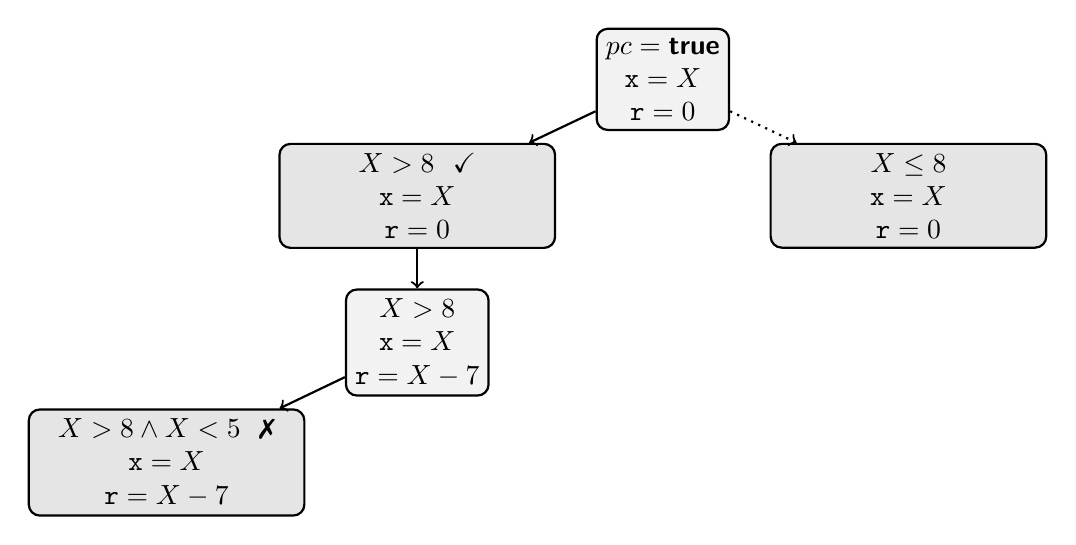
\begin{tikzpicture}[
        node distance=.5cm and .5cm,
        every node/.style={draw, rounded corners, fill=gray!10, align=center},
        every path/.style={thick},
        decision/.style={draw, rounded corners, fill=gray!20, align=center, minimum width=3.5cm}
    ]


    % Nodes
      \node (start) {\textbf{$pc = \textsf{true}$} \\
        $\texttt{x} = X$ \\
        $\texttt{r} = 0$ };
    
    \node (left)[below left=of start, decision,yshift=1em] {$X > 8$~~$\checkmark$ \\ 
        $\texttt{x} = X$ \\
        $\texttt{r} = 0$ };

    \node (left2)[below =of left] {$X > 8$ \\ 
        $\texttt{x} = X$ \\
        $\texttt{r} = X - 7$ };

    \node (ll)[below left =of left2,decision,yshift=1em] {$X > 8 \wedge X < 5$~~\xmark \\ 
        $\texttt{x} = X$ \\
        $\texttt{r} = X - 7$ };
    
    \node (right)[below right=of start, decision,yshift=1em] {$X \leq 8$ \\ 
        $\texttt{x} = X$ \\
        $\texttt{r} = 0$ };

    % Edges
      
    \draw[->] (start) -- (left);
    \draw[->, dotted] (start) -- (right);
    \draw[->] (left) -- (left2);
    \draw[->] (left2) -- (ll);
    
    \end{tikzpicture}
\end{center}
The SMT solver says that the true branch's path condition is unsatisfiable (\xmark): there is no $X$ such that $X > 8$ and $X < 5$. We throw away that state and instead
explore the else branch.
The else branch's path condition is indeed satisfiable ($\checkmark$). The else branch is empty, so we proceed to the return and end that path.
\begin{center}
    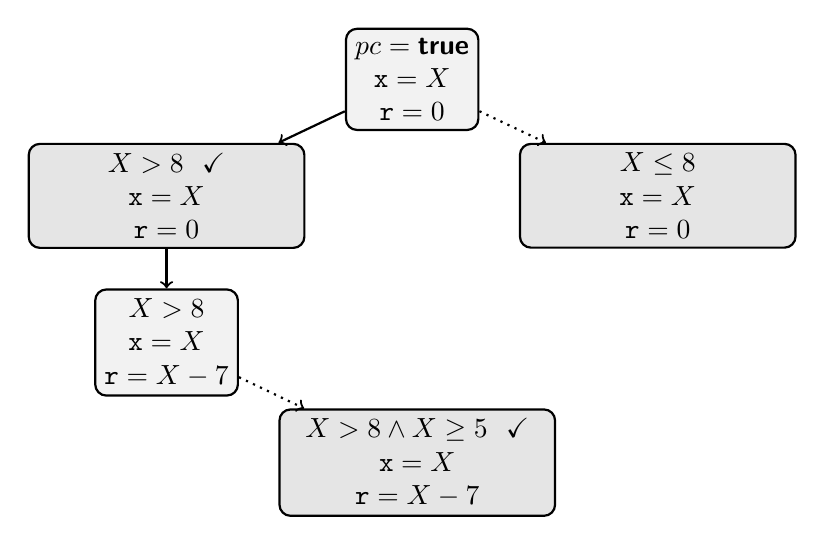
\begin{tikzpicture}[
        node distance=.5cm and .5cm,
        every node/.style={draw, rounded corners, fill=gray!10, align=center},
        every path/.style={thick},
        decision/.style={draw, rounded corners, fill=gray!20, align=center, minimum width=3.5cm}
    ]


    % Nodes
      \node (start) {\textbf{$pc = \textsf{true}$} \\
        $\texttt{x} = X$ \\
        $\texttt{r} = 0$ };
    
    \node (left)[below left=of start, decision,yshift=1em] {$X > 8$~~$\checkmark$ \\ 
        $\texttt{x} = X$ \\
        $\texttt{r} = 0$ };

    \node (left2)[below =of left] {$X > 8$ \\ 
        $\texttt{x} = X$ \\
        $\texttt{r} = X - 7$ };

    \node (ll)[below right =of left2,decision,yshift=1em] {$X > 8 \wedge X \ge 5$~~$\checkmark$ \\ 
        $\texttt{x} = X$ \\
        $\texttt{r} = X - 7$ };
    
    \node (right)[below right=of start, decision,yshift=1em] {$X \leq 8$ \\ 
        $\texttt{x} = X$ \\
        $\texttt{r} = 0$ };

    % Edges
      
    \draw[->] (start) -- (left);
    \draw[->, dotted] (start) -- (right);
    \draw[->] (left) -- (left2);
    \draw[->,dotted] (left2) -- (ll);
    
    \end{tikzpicture}
\end{center}
We continue with the else branch of (1), which proceeds directly to conditional (2).
\begin{center}
    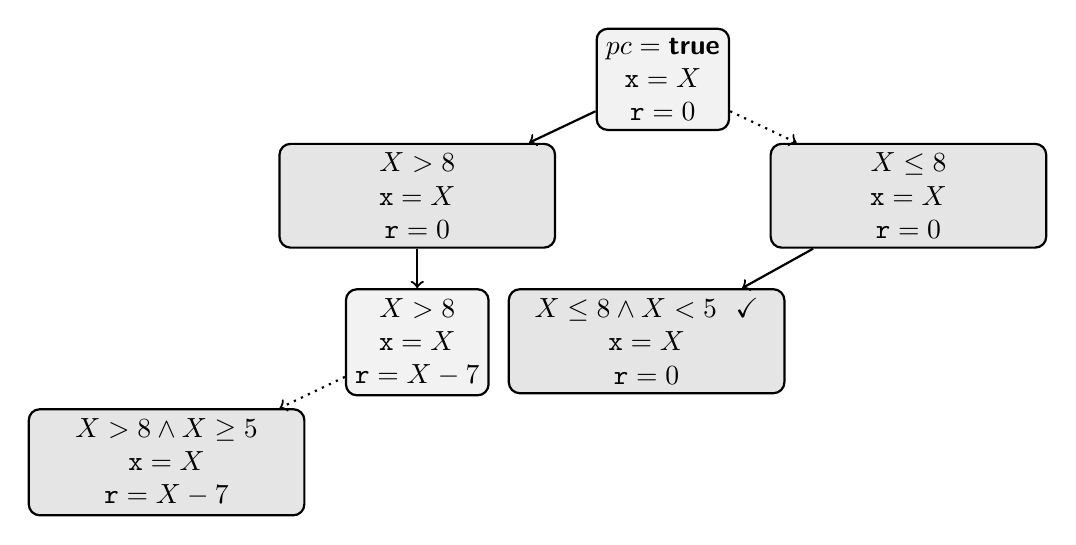
\begin{tikzpicture}[
        node distance=.5cm and .5cm,
        every node/.style={draw, rounded corners, fill=gray!10, align=center},
        every path/.style={thick},
        decision/.style={draw, rounded corners, fill=gray!20, align=center, minimum width=3.5cm}
    ]


    % Nodes
      \node (start) {\textbf{$pc = \textsf{true}$} \\
        $\texttt{x} = X$ \\
        $\texttt{r} = 0$ };
    
    \node (left)[below left=of start, decision,yshift=1em] {$X > 8$ \\ 
        $\texttt{x} = X$ \\
        $\texttt{r} = 0$ };

    \node (left2)[below =of left] {$X > 8$ \\ 
        $\texttt{x} = X$ \\
        $\texttt{r} = X - 7$ };

    \node (ll)[below left =of left2,decision,yshift=1em] {$X > 8 \wedge X \ge 5$ \\ 
        $\texttt{x} = X$ \\
        $\texttt{r} = X - 7$ };
    
    \node (right)[below right=of start, decision,yshift=1em] {$X \leq 8$ \\ 
        $\texttt{x} = X$ \\
        $\texttt{r} = 0$ };
    \node (rl)[below left=of right, decision, xshift=2em] {$X \leq 8 \wedge X < 5$~~$\checkmark$\\
        $\texttt{x} = X$ \\
        $\texttt{r} = 0$ };

    % Edges
      
    \draw[->] (start) -- (left);
    \draw[->, dotted] (start) -- (right);
    \draw[->] (left) -- (left2);
    \draw[->,dotted] (left2) -- (ll);
    \draw[->] (right) -- (rl);
    
    \end{tikzpicture}
\end{center}
The resulting path condition after (1) is false and (2) is true, $X \le 8 \wedge X < 5$, is satisfiable ($\checkmark$). We continue executing the code
in the then-branch and assign to \texttt{r} symbolic value $X-2$.
\begin{center}
    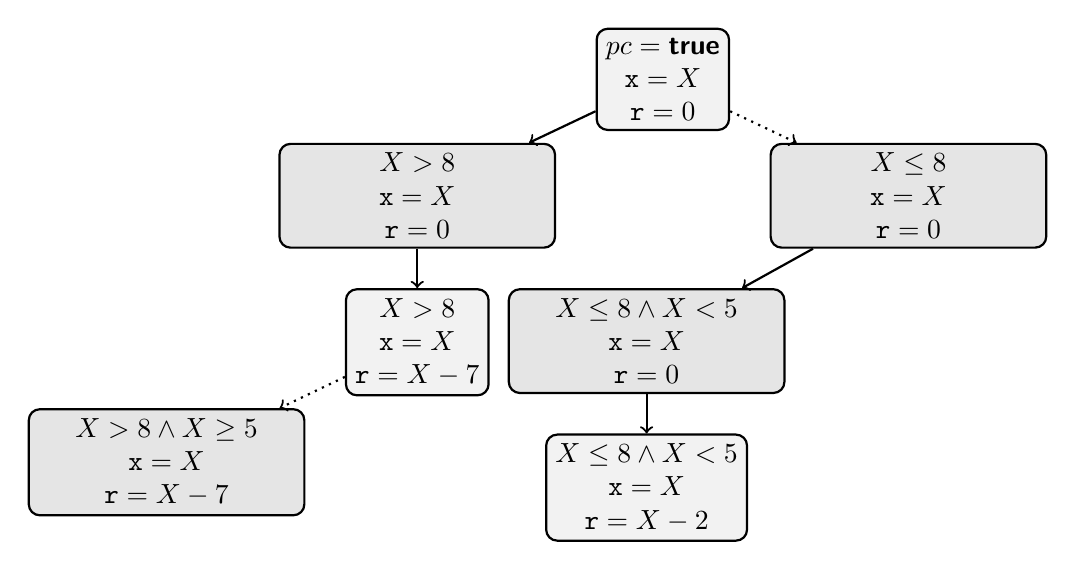
\begin{tikzpicture}[
        node distance=.5cm and .5cm,
        every node/.style={draw, rounded corners, fill=gray!10, align=center},
        every path/.style={thick},
        decision/.style={draw, rounded corners, fill=gray!20, align=center, minimum width=3.5cm}
    ]


    % Nodes
      \node (start) {\textbf{$pc = \textsf{true}$} \\
        $\texttt{x} = X$ \\
        $\texttt{r} = 0$ };
    
    \node (left)[below left=of start, decision,yshift=1em] {$X > 8$ \\ 
        $\texttt{x} = X$ \\
        $\texttt{r} = 0$ };

    \node (left2)[below =of left] {$X > 8$ \\ 
        $\texttt{x} = X$ \\
        $\texttt{r} = X - 7$ };

    \node (ll)[below left =of left2,decision,yshift=1em] {$X > 8 \wedge X \ge 5$ \\ 
        $\texttt{x} = X$ \\
        $\texttt{r} = X - 7$ };
    
    \node (right)[below right=of start, decision,yshift=1em] {$X \leq 8$ \\ 
        $\texttt{x} = X$ \\
        $\texttt{r} = 0$ };
    \node (rl)[below left=of right, decision, xshift=2em] {$X \leq 8 \wedge X < 5$\\
        $\texttt{x} = X$ \\
        $\texttt{r} = 0$ };
    \node (rl2)[below=of rl] {$X \leq 8 \wedge X < 5$\\
        $\texttt{x} = X$ \\
        $\texttt{r} = X-2$ };

    % Edges
      
    \draw[->] (start) -- (left);
    \draw[->, dotted] (start) -- (right);
    \draw[->] (left) -- (left2);
    \draw[->,dotted] (left2) -- (ll);
    \draw[->] (right) -- (rl);
    \draw[->] (rl) -- (rl2);
    
    \end{tikzpicture}
\end{center}
The final path to explore is the else-branch of conditional (2). That path condition,
$X \le 8 \wedge X \ge 5$, is also satisfiable ($\checkmark$).
\begin{center}
    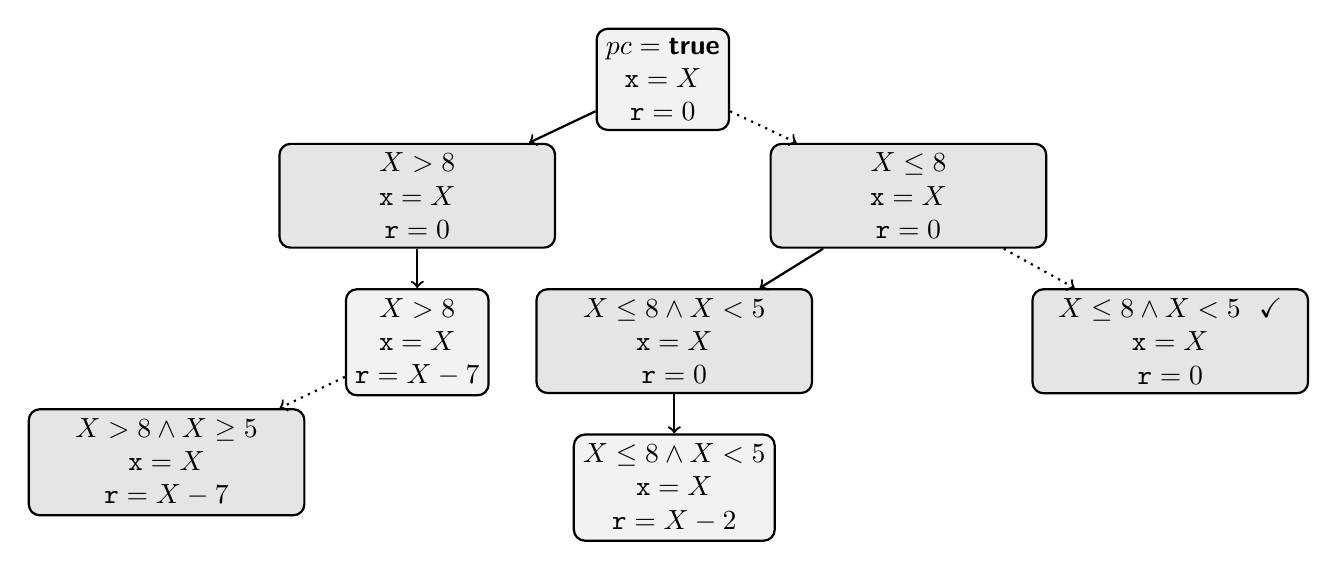
\begin{tikzpicture}[
        node distance=.5cm and .5cm,
        every node/.style={draw, rounded corners, fill=gray!10, align=center},
        every path/.style={thick},
        decision/.style={draw, rounded corners, fill=gray!20, align=center, minimum width=3.5cm}
    ]


    % Nodes
      \node (start) {\textbf{$pc = \textsf{true}$} \\
        $\texttt{x} = X$ \\
        $\texttt{r} = 0$ };
    
    \node (left)[below left=of start, decision,yshift=1em] {$X > 8$ \\ 
        $\texttt{x} = X$ \\
        $\texttt{r} = 0$ };

    \node (left2)[below =of left] {$X > 8$ \\ 
        $\texttt{x} = X$ \\
        $\texttt{r} = X - 7$ };

    \node (ll)[below left =of left2,decision,yshift=1em] {$X > 8 \wedge X \ge 5$ \\ 
        $\texttt{x} = X$ \\
        $\texttt{r} = X - 7$ };
    
    \node (right)[below right=of start, decision,yshift=1em] {$X \leq 8$ \\ 
        $\texttt{x} = X$ \\
        $\texttt{r} = 0$ };
    \node (rl)[below left=of right, decision, xshift=3em] {$X \leq 8 \wedge X < 5$\\
        $\texttt{x} = X$ \\
        $\texttt{r} = 0$ };
    \node (rl2)[below=of rl] {$X \leq 8 \wedge X < 5$\\
        $\texttt{x} = X$ \\
        $\texttt{r} = X-2$ };
    \node (rr)[below right=of right, decision,xshift=-2em] {$X \leq 8 \wedge X < 5$~~$\checkmark$\\
        $\texttt{x} = X$ \\
        $\texttt{r} = 0$ };

    % Edges
      
    \draw[->] (start) -- (left);
    \draw[->, dotted] (start) -- (right);
    \draw[->] (left) -- (left2);
    \draw[->,dotted] (left2) -- (ll);
    \draw[->] (right) -- (rl);
    \draw[->] (rl) -- (rl2);
    \draw[->,dotted] (right) -- (rr);
    
    \end{tikzpicture}
\end{center}
Whenever we had asked the SMT solver whether a path condition was satisfiable, we also requested
a satisfying assignment, which I didn't show you at the time. But some satisfying assignments are,
from left to right, $X = 9$; $X = 4$; $X = 7$, and they induce the test cases \texttt{proc(9)},
\texttt{proc(4)}, and \texttt{proc(7)}. This test suite achieves full path coverage on this function:
it explores all feasible paths from entry to return (not just branches!).

\section*{Defining symbolic execution}
We've seen a couple of examples of symbolic execution.
This technique analyses programs by tracking symbolic values (like $X$
above) rather than actual concrete values; it is thus a form of static
analysis. These symbolic values enable (symbolic) reasoning about
\emph{all} inputs that take the same path through the program, not
just certain concrete values.

Symbolic values stand in for input variables. Programs can operate on
a range of input values, and we don't want to commit to any specific
values at analysis time, so we just leave it symbolic.

\paragraph{Path conditions.} The (symbolic) path conditions characterize what must
hold on a given path, and the symbolic state summarizes the effects
of the execution on all possible program states.

A path condition for a path $P$ is a formula $\mathit{pc}$
such that $\mathit{pc}$ is satisfiable if and only if $P$ is
executable.

In symbolic execution, we use a theorem prover, or a constraint solver (like z3),
to check if a path condition is satisfiable and the path can be taken.

\paragraph{Symbolic state.} A \emph{symbolic state} is a pair $S = (\mathit{Env}, \mathit{pc})$, where:
\begin{itemize}[noitemsep]
\item Environment $\mathit{Env}: L \rightarrow E$ is a mapping from program variables to symbolic expressions (i.e. first-order logic terms);
\item Path condition $\mathit{pc}$ is a first-order logic formula.
\end{itemize}

We had concrete states in the operational semantics. Now we can define when a concrete state $M : L \rightarrow \mathbb{Z}$ satisfies ($\models$) a symbolic state $S = (\mathit{Env}, \mathit{pc})$:
\[ M \models (\mathit{Env}, \mathit{pc}) \mbox{ iff } \left( (\bigwedge_{v \in L} M(v) = \mathit{Env}(v)) \wedge \mbox{$\mathit{pc}$ is SAT} \right) \]

We had the operational semantics on concrete states before. It is possible to extend them to symbolic states. Each program statement updates symbolic variables and the path condition, in a way that is consistent with the operational semantics.

\paragraph{Symbolic state satisfiability.} Let's look at a symbolic state and two concrete states that may or may not satisfy it. Here's the symbolic state.
\[ \mathit{Env} = \left\{ \begin{array}{c} x \mapsto X \\ y \mapsto Y \end{array} \right. \hspace*{2em} \mathit{pc} = X > 5 \wedge Y < 3 \]
Now, what about concrete state
\[ [x \mapsto 10, y \mapsto 1] \models? S \]
Here, $\mathit{Env}$ is saying that $x = X$ and $y = Y$, so we just have concrete path condition $(10 > 5) \wedge (1 < 3)$, which is true, so the concrete state above does satisfy this symbolic state.

For concrete state 
\[ [x \mapsto 1, y \mapsto 10] \models? S \]
we have $(1 > 5) \wedge (10 < 3)$, which is false, so that this concrete state does not satisfy the symbolic state.

A new example of symbolic state (slightly modified from the slides):
\[ \mathit{Env} = \left\{ \begin{array}{c} x \mapsto X + Y \\ y \mapsto Y - X \end{array} \right. \hspace*{2em} \mathit{pc} = 2 * X - Y > 0 \]

Now, what if concrete state was
\[ [x \mapsto 10, y \mapsto 2] \models? S \]
We can use linear algebra on the equations $10 = X + Y$ and $2 = Y - X$ to get $X = 4, Y = 6$. That gives concrete path condition $2 * 4 - 6 > 0$, which evaluates to true, making this concrete
state satisfy the symbolic state. (I think the example in the slides is broken, because we're supposed to be working over integers here, and the example in the slides yields fractions.)

With concrete state
\[ [x \mapsto 2, y \mapsto 10] \models? S \]
linear algebra gives us $X = -8, Y = 6$, so we have path condition $(2 * (-8)) - 6 > 0$, which is false, and so this concrete state does not satisfy the given symbolic state.

\paragraph{Another view of symbolic execution.} Symbolic execution is quite path-based. We can say that symbolic execution creates a functional representation of each path
in the control-flow graph of a program, i.e. under symbolic execution, we view each program path as a function from inputs to outputs.

The domain for path $P_i$, or $D[P_i]$, is the set of inputs that force the program onto path $P_i$.

The program $P$ as a whole can be thought of as a collection of partial functions $P_1, \ldots, P_r$, where each $P_i$ maps some (disjoint) part of the program input to output.
Here's a picture from the slides, though I disagree with partitioning the output space; outputs can be anything. (In math-speak, the function induced by the program need not be injective).

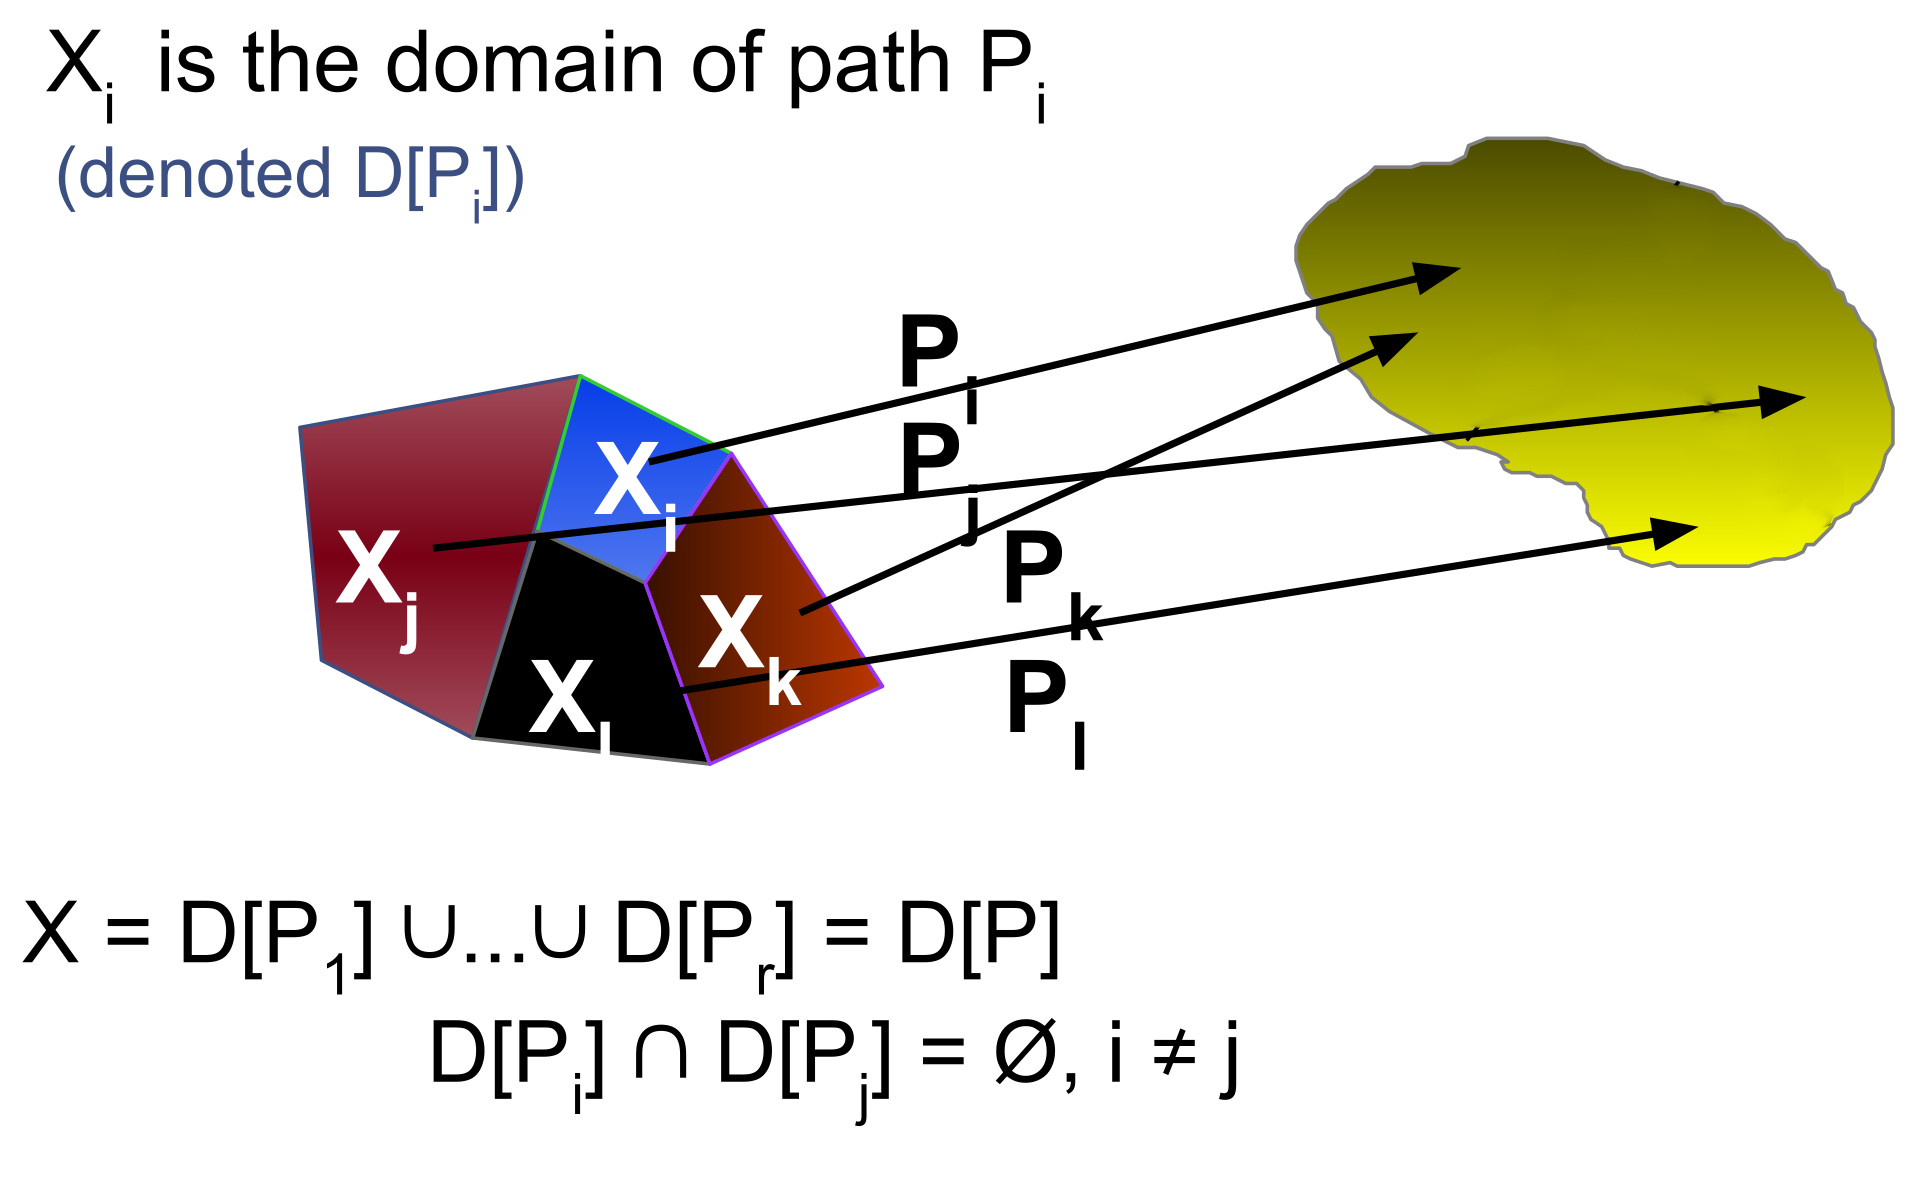
\includegraphics[width=.9\textwidth]{L07/partial-function.png}

\section*{A Third Symbolic Execution Example}
Once again, we can use symbolic execution to find an assertion violation.
\begin{lstlisting}
proc(int a, int b, int c) {
  int x = 0, y = 0, z = 0;
  if (a) { // (1)
    x = -2;
  }
  if (b < 5) { // (2)
    if (!a && c) { // (3)
      y = 1;
    }
    z = 2;
  }
  assert (x + y + z != 3);
}
\end{lstlisting}

We are going to say that $a = A, b = B, c = C$ always, and leave them out of the symbolic state for space reasons. The initial state is:
\begin{center}
    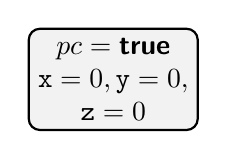
\begin{tikzpicture}[
        node distance=.5cm and .5cm,
        every node/.style={draw, rounded corners, fill=gray!10, align=center},
        every path/.style={thick},
        decision/.style={draw, rounded corners, fill=gray!20, align=center, minimum width=3.5cm}
    ]


    % Nodes
      \node (start) {\textbf{$pc = \textsf{true}$} \\
        $\texttt{x} = 0, \texttt{y} = 0, $ \\
        $\texttt{z} = 0$ };
    
    \end{tikzpicture}
\end{center}

I'm going to combine visiting the true-branch of (1) as well as the true-branch of (2) in the following picture.
Both path conditions $A$ and $A \wedge B < 5$ are satisfiable ($\checkmark$). We can't visit (3)'s true-branch because the
path condition inside that branch, $A \wedge B < 5 \wedge (\neg A \wedge C)$, is unsatisfiable (\xmark).


\begin{center}
    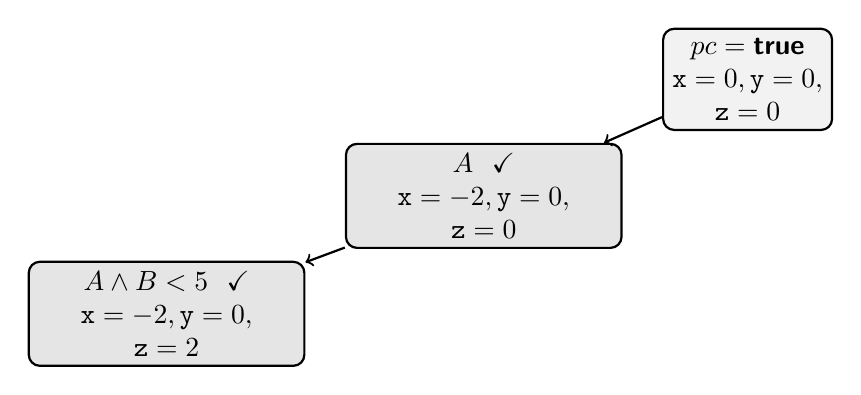
\begin{tikzpicture}[
        node distance=.5cm and .5cm,
        every node/.style={draw, rounded corners, fill=gray!10, align=center},
        every path/.style={thick},
        decision/.style={draw, rounded corners, fill=gray!20, align=center, minimum width=3.5cm}
    ]


    % Nodes
    \node (start) {\textbf{$pc = \textsf{true}$} \\
        $\texttt{x} = 0, \texttt{y} = 0, $ \\
        $\texttt{z} = 0$ };
    
    \node (left)[below left=of start, decision,yshift=1em] {$A$~~$\checkmark$ \\ 
        $\texttt{x} = -2, \texttt{y} = 0, $ \\
        $\texttt{z} = 0$ };
    \node (ll)[below left=of left, decision,yshift=1em] {$A \wedge B < 5$~~$\checkmark$ \\ 
        $\texttt{x} = -2, \texttt{y} = 0, $ \\
        $\texttt{z} = 2$ };

    % Edges
      
    \draw[->] (start) -- (left);
    \draw[->] (left) -- (ll);
    
    \end{tikzpicture}
\end{center}

We can also add the else-branch of (2), which has a satisfiable path condition ($\checkmark$) and has no body.
\begin{center}
    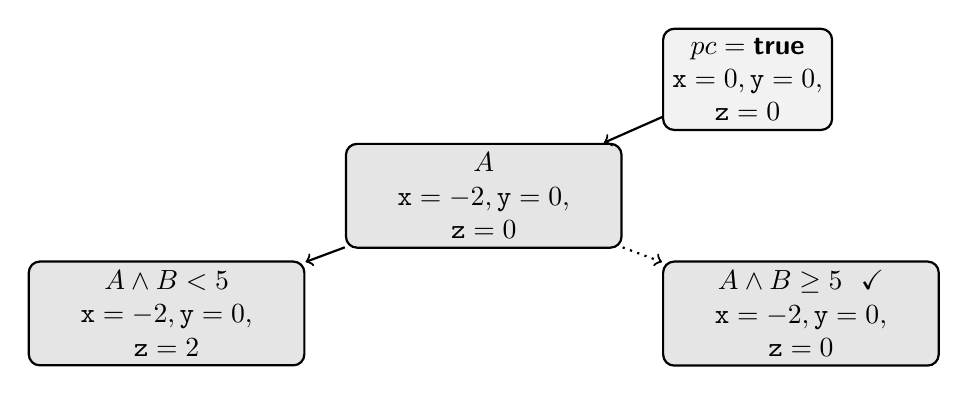
\begin{tikzpicture}[
        node distance=.5cm and .5cm,
        every node/.style={draw, rounded corners, fill=gray!10, align=center},
        every path/.style={thick},
        decision/.style={draw, rounded corners, fill=gray!20, align=center, minimum width=3.5cm}
    ]


    % Nodes
    \node (start) {\textbf{$pc = \textsf{true}$} \\
        $\texttt{x} = 0, \texttt{y} = 0, $ \\
        $\texttt{z} = 0$ };
    
    \node (left)[below left=of start, decision,yshift=1em] {$A$ \\ 
        $\texttt{x} = -2, \texttt{y} = 0, $ \\
        $\texttt{z} = 0$ };
    \node (ll)[below left=of left, decision,yshift=1em] {$A \wedge B < 5$ \\ 
        $\texttt{x} = -2, \texttt{y} = 0, $ \\
        $\texttt{z} = 2$ };
    \node (lr)[below right=of left, decision,yshift=1em] {$A \wedge B \ge 5$~~$\checkmark$ \\ 
        $\texttt{x} = -2, \texttt{y} = 0, $ \\
        $\texttt{z} = 0$ };

    % Edges
      
    \draw[->] (start) -- (left);
    \draw[->] (left) -- (ll);
    \draw[->,dotted] (left) -- (lr);
    
    \end{tikzpicture}
\end{center}
Now we visit the else-branch of (1) and also the else-branch of (2), which yields satisfiable $(\checkmark)$ path condition $\neg A \wedge B \ge 5$. 
\begin{center}
    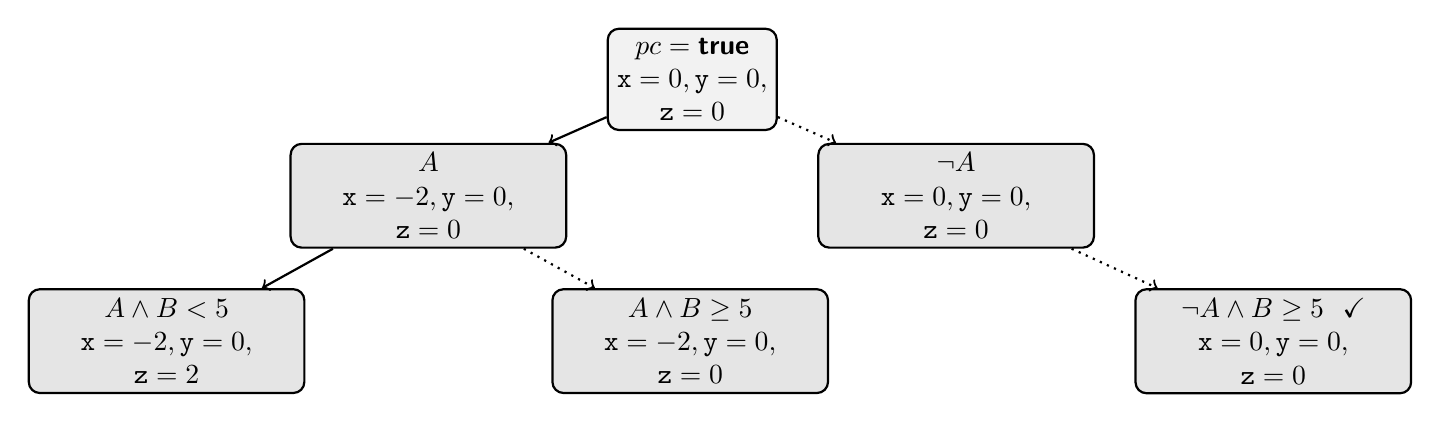
\begin{tikzpicture}[
        node distance=.5cm and .5cm,
        every node/.style={draw, rounded corners, fill=gray!10, align=center},
        every path/.style={thick},
        decision/.style={draw, rounded corners, fill=gray!20, align=center, minimum width=3.5cm}
    ]


    % Nodes
    \node (start) {\textbf{$pc = \textsf{true}$} \\
        $\texttt{x} = 0, \texttt{y} = 0, $ \\
        $\texttt{z} = 0$ };
    
    \node (left)[below left=of start, decision,yshift=1em] {$A$ \\ 
        $\texttt{x} = -2, \texttt{y} = 0, $ \\
        $\texttt{z} = 0$ };
    \node (ll)[below left=of left, decision,xshift=2em] {$A \wedge B < 5$ \\ 
        $\texttt{x} = -2, \texttt{y} = 0, $ \\
        $\texttt{z} = 2$ };
    \node (lr)[below right=of left, decision,xshift=-2em] {$A \wedge B \ge 5$ \\ 
        $\texttt{x} = -2, \texttt{y} = 0, $ \\
        $\texttt{z} = 0$ };

    \node (right)[below right=of start, decision,yshift=1em] {$\neg A$ \\ 
        $\texttt{x} = 0, \texttt{y} = 0, $ \\
        $\texttt{z} = 0$ };
    \node (rr)[below right=of right, decision] {$\neg A \wedge B \ge 5$~~$\checkmark$ \\ 
        $\texttt{x} = 0, \texttt{y} = 0, $ \\
        $\texttt{z} = 0$ };

    % Edges
      
    \draw[->] (start) -- (left);
    \draw[->] (left) -- (ll);
    \draw[->,dotted] (left) -- (lr);
    \draw[->,dotted] (start) -- (right);
    \draw[->,dotted] (right) -- (rr);
    
    \end{tikzpicture}
\end{center}
And there are still unexplored paths through the true-branch of (2) leading to (3), for which we'll explore the else-branch first. This yields satisfiable $(\checkmark)$ path condition $\neg A \wedge B < 5 \wedge \neg C$. (I simplified $\neg (\neg a \wedge c)$ to just $a \vee \neg c$ to get the path condition here).
\begin{center}
    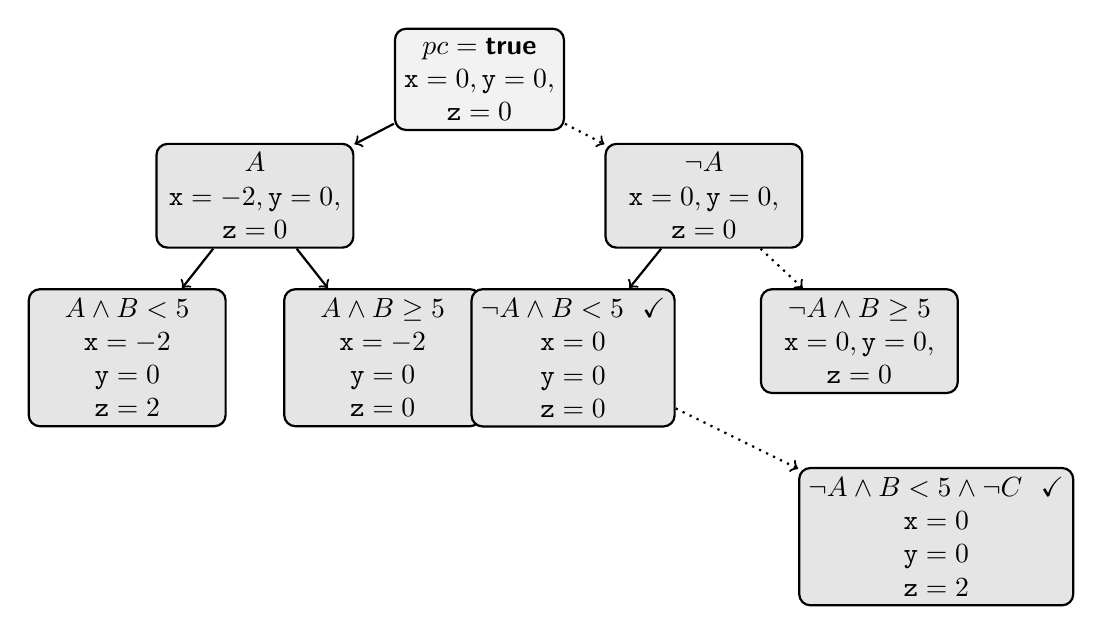
\begin{tikzpicture}[
        node distance=.5cm and .5cm,
        every node/.style={draw, rounded corners, fill=gray!10, align=center},
        every path/.style={thick},
        decision/.style={draw, rounded corners, fill=gray!20, align=center, minimum width=2.5cm}
    ]


    % Nodes
    \node (start) {\textbf{$pc = \textsf{true}$} \\
        $\texttt{x} = 0, \texttt{y} = 0, $ \\
        $\texttt{z} = 0$ };
    
    \node (left)[below left=of start, decision,yshift=1em] {$A$ \\ 
        $\texttt{x} = -2, \texttt{y} = 0, $ \\
        $\texttt{z} = 0$ };
    \node (ll)[below left=of left, decision,xshift=4em] {$A \wedge B < 5$ \\ 
      $\texttt{x} = -2$\\
      $\texttt{y} = 0$ \\
        $\texttt{z} = 2$ };
    \node (lr)[below right=of left, decision,xshift=-4em] {$A \wedge B \ge 5$ \\ 
      $\texttt{x} = -2$\\
      $\texttt{y} = 0 $ \\
        $\texttt{z} = 0$ };

    \node (right)[below right=of start, decision,yshift=1em] {$\neg A$ \\ 
        $\texttt{x} = 0, \texttt{y} = 0, $ \\
        $\texttt{z} = 0$ };
    \node (rl)[below left=of right, decision, xshift=4em] {$\neg A \wedge B < 5$~~$\checkmark$ \\ 
      $\texttt{x} = 0$\\
      $\texttt{y} = 0$ \\
        $\texttt{z} = 0$ };
    \node (rlr)[below right=of rl, decision, xshift=3em] {$\neg A \wedge B < 5 \wedge \neg C$~~$\checkmark$ \\ 
      $\texttt{x} = 0$\\
      $\texttt{y} = 0 $ \\
        $\texttt{z} = 2$ };
    \node (rr)[below right=of right, decision, xshift=-3em] {$\neg A \wedge B \ge 5$ \\ 
        $\texttt{x} = 0, \texttt{y} = 0, $ \\
        $\texttt{z} = 0$ };

    % Edges
      
    \draw[->] (start) -- (left);
    \draw[->] (left) -- (ll);
    \draw[->] (left) -- (lr);
    \draw[->,dotted] (start) -- (right);
    \draw[->,dotted] (right) -- (rr);
    \draw[->] (right) -- (rl);
    \draw[->,dotted] (rl) -- (rlr);
    
    \end{tikzpicture}
\end{center}
Finally, we explore the then-branch of (3), yielding a satisfiable ($\checkmark$) path condition $\neg A \wedge B < 5 \wedge \neg A \wedge C$ (which I've simplified).
\begin{center}
    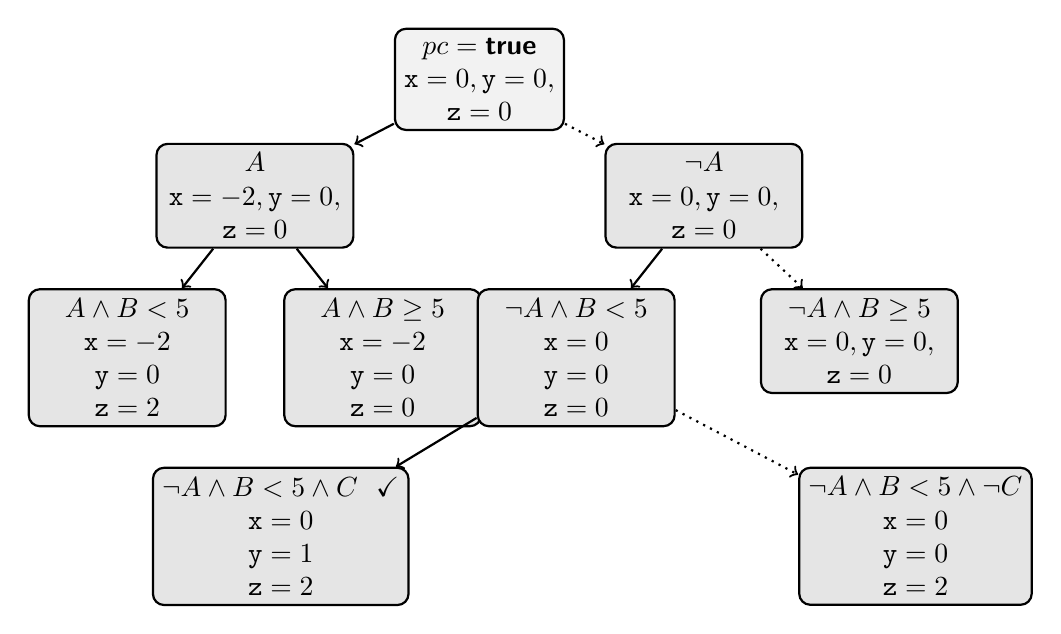
\begin{tikzpicture}[
        node distance=.5cm and .5cm,
        every node/.style={draw, rounded corners, fill=gray!10, align=center},
        every path/.style={thick},
        decision/.style={draw, rounded corners, fill=gray!20, align=center, minimum width=2.5cm}
    ]


    % Nodes
    \node (start) {\textbf{$pc = \textsf{true}$} \\
        $\texttt{x} = 0, \texttt{y} = 0, $ \\
        $\texttt{z} = 0$ };
    
    \node (left)[below left=of start, decision,yshift=1em] {$A$ \\ 
        $\texttt{x} = -2, \texttt{y} = 0, $ \\
        $\texttt{z} = 0$ };
    \node (ll)[below left=of left, decision,xshift=4em] {$A \wedge B < 5$ \\ 
      $\texttt{x} = -2$\\
      $\texttt{y} = 0$ \\
        $\texttt{z} = 2$ };
    \node (lr)[below right=of left, decision,xshift=-4em] {$A \wedge B \ge 5$ \\ 
      $\texttt{x} = -2$\\
      $\texttt{y} = 0 $ \\
        $\texttt{z} = 0$ };

    \node (right)[below right=of start, decision,yshift=1em] {$\neg A$ \\ 
        $\texttt{x} = 0, \texttt{y} = 0, $ \\
        $\texttt{z} = 0$ };
    \node (rl)[below left=of right, decision, xshift=4em] {$\neg A \wedge B < 5$ \\ 
      $\texttt{x} = 0$\\
      $\texttt{y} = 0$ \\
        $\texttt{z} = 0$ };
    \node (rlr)[below right=of rl, decision, xshift=3em] {$\neg A \wedge B < 5 \wedge \neg C$ \\ 
      $\texttt{x} = 0$\\
      $\texttt{y} = 0 $ \\
        $\texttt{z} = 2$ };
    \node (rll)[below left=of rl, decision, xshift=-1em] {$\neg A \wedge B < 5 \wedge C$~~$\checkmark$ \\ 
      $\texttt{x} = 0$\\
      $\texttt{y} = 1 $ \\
        $\texttt{z} = 2$ };
    \node (rr)[below right=of right, decision, xshift=-3em] {$\neg A \wedge B \ge 5$ \\ 
        $\texttt{x} = 0, \texttt{y} = 0, $ \\
        $\texttt{z} = 0$ };

    % Edges
      
    \draw[->] (start) -- (left);
    \draw[->] (left) -- (ll);
    \draw[->] (left) -- (lr);
    \draw[->,dotted] (start) -- (right);
    \draw[->,dotted] (right) -- (rr);
    \draw[->] (right) -- (rl);
    \draw[->,dotted] (rl) -- (rlr);
    \draw[->] (rl) -- (rll);
    
    \end{tikzpicture}
\end{center}
This path fails the assert. We can ask the SMT solver to find a test case that violates the assertion, which is $A$ false, $B=4$, and $C$ true,
yielding $x = 0, y = 1, z = 2$, so that the assert is checking $0 + 1 + 2 \neq 3$, which fails as desired.

\section*{Finding Bugs using Symbolic Execution}
We've seen that symbolic execution enumerates paths. It will therefore find bugs that trigger when a specific path executes. That's not quite enough on its own, though.
We saw how we rewrote programs to use specific asserts, as in the division by zero example. In general, finding a bug requires finding the conditions that trigger it.
Bugs include assertion failures, buffer overflows, division by zero, etc.

We go one more step beyond just having asserts, and compile these assertions into conditionals. This treats assertions as conditions and creates explicit error paths. Since
we are exploring all paths, we will explore the error path (containing an \texttt{error()} call) if it is reachable.

So, we compile from
\begin{center}
  \texttt{assert x != NULL}
\end{center}
into
\begin{center}
  \texttt{if (x == NULL)}\\
  \texttt{~~~~error();}
\end{center}
and show that the \texttt{error()} call is reachable or unreachable.

The rewriting process, or instrumenting the programs with properties, can
translate any safety property (``bad things don't happen'') into
reachability (of an \texttt{error()} call). There is some similarity
to fuzzing.

Rewriting can be explicit or implicit. For explicit rewriting, this is like
sanitizers, and we instrument the code with checks. But the symbolic engine
can also implicitly inject extra checks at runtime.

Checks might look like this:
\begin{eqnarray*}
 \texttt{y = 100 / x} &\Rightarrow& \texttt{assert x != 0; y = 100/x} \mbox{ (division by zero)}\\
 \texttt{a[x] = 10} &\Rightarrow& \texttt{assert x >= 0 \&\& x < len(a)} \mbox{ (array bounds)}
\end{eqnarray*}

\section*{Problems of (Classical) Symbolic Execution}
Of course, I've shown you cases where symbolic execution works. This isn't real code. What happens for real?

Some code is hard to analyze. Even if it generates innocuous-looking constraints, the resulting constraints might be beyond the abilities of our SMT solvers. And cryptographic hashes are definitely hard to invert.

There's also the path explosion problem. The number of paths in the program is exponential in the size of the program. Control flow, loops, procedures, concurrency, etc can cause lots of paths.

And, to analyze real code, you need to work with more than just integers.
There are pointers and data structures; files and databases; networks and sockets; and threads and thread schedules, among other things. There has to be some way of handling these. 
Which is why we'll talk about dynamic symbolic execution soon.


\bibliographystyle{alpha}
\bibliography{L07}

\end{document}
